\section{Technologie na serverové straně}
\subsection{Python}
Jak se uvádí na českých stránkách programovacího jazyka Python \cite{python-cz}:

\begin{center}
\textit{Python je moderní programovací jazyk. Je univerzální – pohání weby i rakety. Dobře se čte a dá se velice rychle naučit. Je skvělý pro výuku programování. Česká komunita je aktivní. Najdeš v ní pomoc, kamarády i práci.}
\end{center}

\subsection{Django}
http://djangobook.com/introducing-django/
Po domluvě s vedoucím práce jsem se rozhodl pro použití frameworku Django, což je nejpoužívanější webový framework napsaný v jazyku Python. Několik konkrétních částí frameworku popíšu v následujících sekcích.

\subsubsection{Šablonovací systém}
Django ve výchozím nastavení používá vlastní šablonovací systém s kreativním názvem \textbf{Django template system}. Poskytuje spoustu funkcí, které velmi usnadňují vývoj. Za zmínku určitě stojí možnost dědit šablony, automatické escapování proměnných a nebo třeba velké množství filtrů. Příklad použití šablon lze vidět na ukázce \ref{code:django-template}.

\begin{listing}[htbp]
\caption{\label{code:django-template}Ukázka šablony ve frameworku Django}
\begin{minted}[frame=lines,bgcolor=codebg,fontsize=\footnotesize,linenos,breaklines]{HTML}



<!DOCTYPE html>
<html lang="en">
<head>
    <meta charset="utf-8">
    <title>MicroXchange {{ global }}</title>
    <link href="" rel="stylesheet"/>
</head>
<body>
    <h1>Homepage</h1>
    <p>Mauris blandit aliquet elit, eget tincidunt nibh pulvinar a. Donec sollicitudin molestie malesuada. Curabitur aliquet quam id dui posuere blandit. Vestibulum ac diam sit amet quam vehicula elementum sed sit amet dui.</p>
</body>
</html>
\end{minted}
\end{listing}

\subsubsection{Modelové třídy}

\paragraph*{Currency} představuje měnu, ze které, respektive do které, lze směnit peníze. Obsahuje název, identifikátor, prefix a postfix.
\paragraph*{CurrencyRates} představuje kurz mezi dvěma měnami. Obsahuje měnu z, měnu do a daný kurz, který se aktualizuje každou hodinu pomocí služby \textbf{fixer.io}.
\paragraph*{OfferStatus} - představuje status objednávky, momentálně je jich 5:
\begin{itemize}
    \item \textbf{Awaiting acceptance} - nabídka čekající na uživatele, který chce směnit peníze
    \item \textbf{Awaiting approval} - nabídka již má oba uživatele směny a momentálně čeká na schválení uživatele uživatelem, který nabídku vytvořil
    \item \textbf{Ready to exchange} - v tomto momentě jsou zobrazeny kontaktní údaje a uživatele se domlouvají na směně
    \item \textbf{Finished} - nabídka je kompletní
    \item \textbf{Deleted} - nabídka byla smazána uživatelem, který ji vytvořil
\end{itemize}

Jak lze přecházet ze stavu do stavu znázorňuje stavový diagram \ref{fig:implementation:state-diagram}.

\begin{figure}[h]
    \centering
    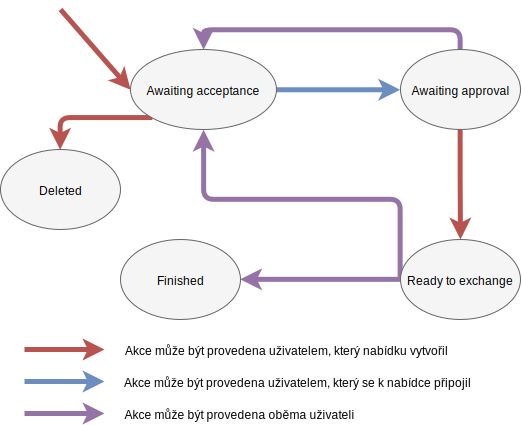
\includegraphics[width=1.0\textwidth]{media/state-diagram}
    \caption{Stavový diagram nabídky}
    \label{fig:implementation:state-diagram}
\end{figure}

\paragraph*{Offer} třída představující nabídku na směnu peněz. Obsahuje obě měny, status, oba uživatele, adresu, rádius, souřadnice, množství peněz, kurz, komentář k nabídce, čas vytvoření a čas poslední aktualizace.
\paragraph*{Feedback} představuje hodnocení uživatele za danou nabídku. Obsahuje tedy odkaz na nabídku, uživatele, který hodnocení přidal, komentář, počet hvězdiček a čas vytvoření hodnocení.
\paragraph*{Language} představuje jazyk, do kterého je možné aplikaci přeložit
\paragraph*{UserProfile} obohacuje třídu výchozího uživatele o tyto parametry: profilový obrázek, domácí měna, druhá měna, preferovaný jazyk, základní textová informace o uživateli, email, telefon, adresa, rádius a souřadnice.

\subsubsection{Pohledy}
Pohledy jsou vrstva aplikace stojící mezi šablonovou a modelovou vrstvou. Jejich práce je získávání dat od uživatele, jejich následné zpracování pomocí modelových tříd a následné předání potřebných dat do šablon.

\subsubsection{Lokalizace do jiných jazyků}
Django poskytuje podporu pro lokalizaci aplikace do jiných jazyků. Použití je velmi jednoduché:
\begin{enumerate}
    \item Vše, co by mělo být lokalizováno stačí předat do funkce \\\texttt{django.utils.translation.ugettext}. V šablonách lze použít tag \\\mbox{\texttt{\{\% trans \%\}}}.
    \item Pomocí příkazu \texttt{django-admin makemessages -l en} se vytvoří soubor s příponou \texttt{.po}, do kterého se vloží všechny potřebné řetězce, které je potřeba přeložit.
    \item Po vyplnění veškerých překladů je potřeba vytvořit soubor s příponou pomocí \texttt{.mo} příkazu \texttt{django-admin compilemessages}.
    \item Daný jazyk se pak v aplikaci nastaví pomocí zavolání funkce \\\texttt{django.utils.translation.activate('cs')}.
\end{enumerate}

Django dále automaticky při prvním přístupu uživatele na web nastaví uživateli jazyk, který preferuje. Což pozná podle HTTP hlavičky \\\texttt{Accept-Language}.

\subsubsection{Přihlašování přes Facebook}
Jedním z požadavků na aplikaci bylo přihlášení pomocí sociální sítě Facebook. To Django přímo nepodporuje, ale existuje balíček Python Social Auth \cite{python-social-auth}. Ten poskytuje autentizační a autorizační mechanismy pro několik frameworků a několik služeb, přes které se lze přihlásit.
\\\\
Implementace je pak velmi jednoduchá:
\begin{enumerate}
    \item Nejprve je potřeba vytvořit aplikaci na stránka Facebook for Developers \cite{facebook-developers}, pomocí které bude probíhat přihlašování uživatelů.
    \item Poté je potřeba do souboru \texttt{settings.py} přidat několik důležitých konfiguračních parametrů. Viz ukázka kódu \ref{code:facebook-settings}.
    \item Následuje definice url adres. Do souboru \texttt{urls.py} je potřeba přidat tento řádek:\\\texttt{url('', include('social\_django.urls', namespace='social'))}.
    \item Poté je nutné spustit migrace databáze pomocí \\\texttt{python manage.py migrate}.
    \item Poté v šabloně vytvoříme odkaz, pomocí kterého se budou uživatelé přihlašovat.
\end{enumerate}

\begin{listing}[h]
\caption{\label{code:facebook-settings}Konfigurace přihlášení přes Facebook}
\begin{minted}[frame=lines,bgcolor=codebg,fontsize=\footnotesize,linenos,breaklines]{Python}
AUTHENTICATION_BACKENDS = (
    'django.contrib.auth.backends.ModelBackend',
    'social_core.backends.facebook.FacebookOAuth2',
)

SOCIAL_AUTH_FACEBOOK_KEY = 'key12345'
SOCIAL_AUTH_FACEBOOK_SECRET = 'secter12345'
SOCIAL_AUTH_FACEBOOK_SCOPE = ['email']
SOCIAL_AUTH_FACEBOOK_PROFILE_EXTRA_PARAMS = {
    'locale': 'cs_CZ',
    'fields': 'id, name, email, age_range'
}

SOCIAL_AUTH_PIPELINE = (
    'social_core.pipeline.social_auth.social_details',
    'social_core.pipeline.social_auth.social_uid',
    'social_core.pipeline.social_auth.auth_allowed',
    'social_core.pipeline.social_auth.social_user',
    'social_core.pipeline.user.get_username',
    'social_core.pipeline.social_auth.associate_by_email',
    'social_core.pipeline.user.create_user',
    'web.pipeline.save_profile_picture',
    'web.pipeline.save_preferences_to_session',
    'social_core.pipeline.social_auth.associate_user',
    'social_core.pipeline.social_auth.load_extra_data',
    'social_core.pipeline.user.user_details'
)
\end{minted}
\end{listing}


\subsection{Aktualizace kurzů}
Aktualizace kurzů probíhá vždy jednou za hodinu, a to pomocí služby Fixer.io \cite{fixer-io}. Ukázku požadavku a odpovědi serveru lze najít v ukázce \ref{code:fixer-io}. Kurzy měn se poté ukládají do databáze.

\begin{listing}[h]
\caption{\label{code:fixer-io}Služba Fixer.io - Ukázka požadavku a odpovědi}
\begin{minted}[frame=lines,bgcolor=codebg,fontsize=\footnotesize,linenos,breaklines]{Python}
GET http://api.fixer.io/latest?symbols=USD,GBP&base=EUR
{
    "base": "EUR",
    "date": "2017-04-20",
    "rates": {
        "GBP": 0.8392,
        "USD": 1.0745
    }
}
\end{minted}
\end{listing}
